\documentclass[11pt]{article}

    \usepackage[breakable]{tcolorbox}
    \usepackage{parskip} % Stop auto-indenting (to mimic markdown behaviour)
    
    \usepackage{float}
    

    % Basic figure setup, for now with no caption control since it's done
    % automatically by Pandoc (which extracts ![](path) syntax from Markdown).
    \usepackage{graphicx}
    % Maintain compatibility with old templates. Remove in nbconvert 6.0
    \let\Oldincludegraphics\includegraphics
    % Ensure that by default, figures have no caption (until we provide a
    % proper Figure object with a Caption API and a way to capture that
    % in the conversion process - todo).
    \usepackage{caption}
    \DeclareCaptionFormat{nocaption}{}
    \captionsetup{format=nocaption,aboveskip=0pt,belowskip=0pt}

    \usepackage{float}
    \floatplacement{figure}{H} % forces figures to be placed at the correct 
    \usepackage{xcolor} % Allow colors to be definedhttps://www.overleaf.com/project/656f71089648add9d3ede67e
    \usepackage{enumerate} % Needed for markdown enumerations to work
    \usepackage{geometry} % Used to adjust the document margins
    \usepackage{amsmath} % Equations
    \usepackage{amssymb} % Equations
    \usepackage{textcomp} % defines textquotesingle
    % Hack from http://tex.stackexchange.com/a/47451/13684:
    \AtBeginDocument{%
        \def\PYZsq{\textquotesingle}% Upright quotes in Pygmentized code
    }
    \usepackage{upquote} % Upright quotes for verbatim code
    \usepackage{eurosym} % defines \euro

    \usepackage{iftex}
    \ifPDFTeX
        \usepackage[T1]{fontenc}
        \IfFileExists{alphabeta.sty}{
              \usepackage{alphabeta}
          }{
              \usepackage[mathletters]{ucs}
              \usepackage[utf8x]{inputenc}
          }
    \else
        \usepackage{fontspec}
        \usepackage{unicode-math}
    \fi

    \usepackage{fancyvrb} % verbatim replacement that allows latex
    \usepackage{grffile} % extends the file name processing of package graphics
                         % to support a larger range
    \makeatletter % fix for old versions of grffile with XeLaTeX
    \@ifpackagelater{grffile}{2019/11/01}
    {
      % Do nothing on new versions
    }
    {
      \def\Gread@@xetex#1{%
        \IfFileExists{"\Gin@base".bb}%
        {\Gread@eps{\Gin@base.bb}}%
        {\Gread@@xetex@aux#1}%
      }
    }
    \makeatother
    \usepackage[Export]{adjustbox} % Used to constrain images to a maximum size
    \adjustboxset{max size={0.9\linewidth}{0.9\paperheight}}

    % The hyperref package gives us a pdf with properly built
    % internal navigation ('pdf bookmarks' for the table of contents,
    % internal cross-reference links, web links for URLs, etc.)
    \usepackage{hyperref}
    % The default LaTeX title has an obnoxious amount of whitespace. By default,
    % titling removes some of it. It also provides customization options.
    \usepackage{titling}
    \usepackage{longtable} % longtable support required by pandoc >1.10
    \usepackage{booktabs}  % table support for pandoc > 1.12.2
    \usepackage{array}     % table support for pandoc >= 2.11.3
    \usepackage{calc}      % table minipage width calculation for pandoc >= 2.11.1
    \usepackage[inline]{enumitem} % IRkernel/repr support (it uses the enumerate* environment)
    \usepackage[normalem]{ulem} % ulem is needed to support strikethroughs (\sout)
                                % normalem makes italics be italics, not underlines
    \usepackage{mathrsfs}
    

    
    % Colors for the hyperref package
    \definecolor{urlcolor}{rgb}{0,.145,.698}
    \definecolor{linkcolor}{rgb}{.71,0.21,0.01}
    \definecolor{citecolor}{rgb}{.12,.54,.11}

    % ANSI colors
    \definecolor{ansi-black}{HTML}{3E424D}
    \definecolor{ansi-black-intense}{HTML}{282C36}
    \definecolor{ansi-red}{HTML}{E75C58}
    \definecolor{ansi-red-intense}{HTML}{B22B31}
    \definecolor{ansi-green}{HTML}{00A250}
    \definecolor{ansi-green-intense}{HTML}{007427}
    \definecolor{ansi-yellow}{HTML}{DDB62B}
    \definecolor{ansi-yellow-intense}{HTML}{B27D12}
    \definecolor{ansi-blue}{HTML}{208FFB}
    \definecolor{ansi-blue-intense}{HTML}{0065CA}
    \definecolor{ansi-magenta}{HTML}{D160C4}
    \definecolor{ansi-magenta-intense}{HTML}{A03196}
    \definecolor{ansi-cyan}{HTML}{60C6C8}
    \definecolor{ansi-cyan-intense}{HTML}{258F8F}
    \definecolor{ansi-white}{HTML}{C5C1B4}
    \definecolor{ansi-white-intense}{HTML}{A1A6B2}
    \definecolor{ansi-default-inverse-fg}{HTML}{FFFFFF}
    \definecolor{ansi-default-inverse-bg}{HTML}{000000}

    % common color for the border for error outputs.
    \definecolor{outerrorbackground}{HTML}{FFDFDF}

    % commands and environments needed by pandoc snippets
    % extracted from the output of `pandoc -s`
    \providecommand{\tightlist}{%
      \setlength{\itemsep}{0pt}\setlength{\parskip}{0pt}}
    \DefineVerbatimEnvironment{Highlighting}{Verbatim}{commandchars=\\\{\}}
    % Add ',fontsize=\small' for more characters per line
    \newenvironment{Shaded}{}{}
    \newcommand{\KeywordTok}[1]{\textcolor[rgb]{0.00,0.44,0.13}{\textbf{{#1}}}}
    \newcommand{\DataTypeTok}[1]{\textcolor[rgb]{0.56,0.13,0.00}{{#1}}}
    \newcommand{\DecValTok}[1]{\textcolor[rgb]{0.25,0.63,0.44}{{#1}}}
    \newcommand{\BaseNTok}[1]{\textcolor[rgb]{0.25,0.63,0.44}{{#1}}}
    \newcommand{\FloatTok}[1]{\textcolor[rgb]{0.25,0.63,0.44}{{#1}}}
    \newcommand{\CharTok}[1]{\textcolor[rgb]{0.25,0.44,0.63}{{#1}}}
    \newcommand{\StringTok}[1]{\textcolor[rgb]{0.25,0.44,0.63}{{#1}}}
    \newcommand{\CommentTok}[1]{\textcolor[rgb]{0.38,0.63,0.69}{\textit{{#1}}}}
    \newcommand{\OtherTok}[1]{\textcolor[rgb]{0.00,0.44,0.13}{{#1}}}
    \newcommand{\AlertTok}[1]{\textcolor[rgb]{1.00,0.00,0.00}{\textbf{{#1}}}}
    \newcommand{\FunctionTok}[1]{\textcolor[rgb]{0.02,0.16,0.49}{{#1}}}
    \newcommand{\RegionMarkerTok}[1]{{#1}}
    \newcommand{\ErrorTok}[1]{\textcolor[rgb]{1.00,0.00,0.00}{\textbf{{#1}}}}
    \newcommand{\NormalTok}[1]{{#1}}

    % Additional commands for more recent versions of Pandoc
    \newcommand{\ConstantTok}[1]{\textcolor[rgb]{0.53,0.00,0.00}{{#1}}}
    \newcommand{\SpecialCharTok}[1]{\textcolor[rgb]{0.25,0.44,0.63}{{#1}}}
    \newcommand{\VerbatimStringTok}[1]{\textcolor[rgb]{0.25,0.44,0.63}{{#1}}}
    \newcommand{\SpecialStringTok}[1]{\textcolor[rgb]{0.73,0.40,0.53}{{#1}}}
    \newcommand{\ImportTok}[1]{{#1}}
    \newcommand{\DocumentationTok}[1]{\textcolor[rgb]{0.73,0.13,0.13}{\textit{{#1}}}}
    \newcommand{\AnnotationTok}[1]{\textcolor[rgb]{0.38,0.63,0.69}{\textbf{\textit{{#1}}}}}
    \newcommand{\CommentVarTok}[1]{\textcolor[rgb]{0.38,0.63,0.69}{\textbf{\textit{{#1}}}}}
    \newcommand{\VariableTok}[1]{\textcolor[rgb]{0.10,0.09,0.49}{{#1}}}
    \newcommand{\ControlFlowTok}[1]{\textcolor[rgb]{0.00,0.44,0.13}{\textbf{{#1}}}}
    \newcommand{\OperatorTok}[1]{\textcolor[rgb]{0.40,0.40,0.40}{{#1}}}
    \newcommand{\BuiltInTok}[1]{{#1}}
    \newcommand{\ExtensionTok}[1]{{#1}}
    \newcommand{\PreprocessorTok}[1]{\textcolor[rgb]{0.74,0.48,0.00}{{#1}}}
    \newcommand{\AttributeTok}[1]{\textcolor[rgb]{0.49,0.56,0.16}{{#1}}}
    \newcommand{\InformationTok}[1]{\textcolor[rgb]{0.38,0.63,0.69}{\textbf{\textit{{#1}}}}}
    \newcommand{\WarningTok}[1]{\textcolor[rgb]{0.38,0.63,0.69}{\textbf{\textit{{#1}}}}}


    % Define a nice break command that doesn't care if a line doesn't already
    % exist.
    \def\br{\hspace*{\fill} \\* }
    % Math Jax compatibility definitions
    \def\gt{>}
    \def\lt{<}
    \let\Oldtex\TeX
    \let\Oldlatex\LaTeX
    \renewcommand{\TeX}{\textrm{\Oldtex}}
    \renewcommand{\LaTeX}{\textrm{\Oldlatex}}

\title{Which Neighborhood in Atlanta is Best for a Metal Music Venue Business? \\
Considering Transportation, Demographic, and Urban Planning Factors\\
\large CP6542: Transport and GIS Final Report\\
}


\author{Tingyu Liu}




\begin{titlepage}
    \centering
    \vspace*{1cm}
    \Huge \textbf{\thetitle}  % Using \thetitle to access the previously defined title


    \vspace{0.5cm}
    \Large \theauthor{}  % Using \theauthor to access the previously defined author


    \vspace{0.5cm}
    \Large {Instructor: Yiyi He\\
    GitHub: https://github.com/drunken-boat/livehouse-atl
    }
    \vspace{0.5cm}
    
    
    

\end{titlepage}
    

    
    
    
    
% Pygments definitions
\makeatletter
\def\PY@reset{\let\PY@it=\relax \let\PY@bf=\relax%
    \let\PY@ul=\relax \let\PY@tc=\relax%
    \let\PY@bc=\relax \let\PY@ff=\relax}
\def\PY@tok#1{\csname PY@tok@#1\endcsname}
\def\PY@toks#1+{\ifx\relax#1\empty\else%
    \PY@tok{#1}\expandafter\PY@toks\fi}
\def\PY@do#1{\PY@bc{\PY@tc{\PY@ul{%
    \PY@it{\PY@bf{\PY@ff{#1}}}}}}}
\def\PY#1#2{\PY@reset\PY@toks#1+\relax+\PY@do{#2}}

\@namedef{PY@tok@w}{\def\PY@tc##1{\textcolor[rgb]{0.73,0.73,0.73}{##1}}}
\@namedef{PY@tok@c}{\let\PY@it=\textit\def\PY@tc##1{\textcolor[rgb]{0.24,0.48,0.48}{##1}}}
\@namedef{PY@tok@cp}{\def\PY@tc##1{\textcolor[rgb]{0.61,0.40,0.00}{##1}}}
\@namedef{PY@tok@k}{\let\PY@bf=\textbf\def\PY@tc##1{\textcolor[rgb]{0.00,0.50,0.00}{##1}}}
\@namedef{PY@tok@kp}{\def\PY@tc##1{\textcolor[rgb]{0.00,0.50,0.00}{##1}}}
\@namedef{PY@tok@kt}{\def\PY@tc##1{\textcolor[rgb]{0.69,0.00,0.25}{##1}}}
\@namedef{PY@tok@o}{\def\PY@tc##1{\textcolor[rgb]{0.40,0.40,0.40}{##1}}}
\@namedef{PY@tok@ow}{\let\PY@bf=\textbf\def\PY@tc##1{\textcolor[rgb]{0.67,0.13,1.00}{##1}}}
\@namedef{PY@tok@nb}{\def\PY@tc##1{\textcolor[rgb]{0.00,0.50,0.00}{##1}}}
\@namedef{PY@tok@nf}{\def\PY@tc##1{\textcolor[rgb]{0.00,0.00,1.00}{##1}}}
\@namedef{PY@tok@nc}{\let\PY@bf=\textbf\def\PY@tc##1{\textcolor[rgb]{0.00,0.00,1.00}{##1}}}
\@namedef{PY@tok@nn}{\let\PY@bf=\textbf\def\PY@tc##1{\textcolor[rgb]{0.00,0.00,1.00}{##1}}}
\@namedef{PY@tok@ne}{\let\PY@bf=\textbf\def\PY@tc##1{\textcolor[rgb]{0.80,0.25,0.22}{##1}}}
\@namedef{PY@tok@nv}{\def\PY@tc##1{\textcolor[rgb]{0.10,0.09,0.49}{##1}}}
\@namedef{PY@tok@no}{\def\PY@tc##1{\textcolor[rgb]{0.53,0.00,0.00}{##1}}}
\@namedef{PY@tok@nl}{\def\PY@tc##1{\textcolor[rgb]{0.46,0.46,0.00}{##1}}}
\@namedef{PY@tok@ni}{\let\PY@bf=\textbf\def\PY@tc##1{\textcolor[rgb]{0.44,0.44,0.44}{##1}}}
\@namedef{PY@tok@na}{\def\PY@tc##1{\textcolor[rgb]{0.41,0.47,0.13}{##1}}}
\@namedef{PY@tok@nt}{\let\PY@bf=\textbf\def\PY@tc##1{\textcolor[rgb]{0.00,0.50,0.00}{##1}}}
\@namedef{PY@tok@nd}{\def\PY@tc##1{\textcolor[rgb]{0.67,0.13,1.00}{##1}}}
\@namedef{PY@tok@s}{\def\PY@tc##1{\textcolor[rgb]{0.73,0.13,0.13}{##1}}}
\@namedef{PY@tok@sd}{\let\PY@it=\textit\def\PY@tc##1{\textcolor[rgb]{0.73,0.13,0.13}{##1}}}
\@namedef{PY@tok@si}{\let\PY@bf=\textbf\def\PY@tc##1{\textcolor[rgb]{0.64,0.35,0.47}{##1}}}
\@namedef{PY@tok@se}{\let\PY@bf=\textbf\def\PY@tc##1{\textcolor[rgb]{0.67,0.36,0.12}{##1}}}
\@namedef{PY@tok@sr}{\def\PY@tc##1{\textcolor[rgb]{0.64,0.35,0.47}{##1}}}
\@namedef{PY@tok@ss}{\def\PY@tc##1{\textcolor[rgb]{0.10,0.09,0.49}{##1}}}
\@namedef{PY@tok@sx}{\def\PY@tc##1{\textcolor[rgb]{0.00,0.50,0.00}{##1}}}
\@namedef{PY@tok@m}{\def\PY@tc##1{\textcolor[rgb]{0.40,0.40,0.40}{##1}}}
\@namedef{PY@tok@gh}{\let\PY@bf=\textbf\def\PY@tc##1{\textcolor[rgb]{0.00,0.00,0.50}{##1}}}
\@namedef{PY@tok@gu}{\let\PY@bf=\textbf\def\PY@tc##1{\textcolor[rgb]{0.50,0.00,0.50}{##1}}}
\@namedef{PY@tok@gd}{\def\PY@tc##1{\textcolor[rgb]{0.63,0.00,0.00}{##1}}}
\@namedef{PY@tok@gi}{\def\PY@tc##1{\textcolor[rgb]{0.00,0.52,0.00}{##1}}}
\@namedef{PY@tok@gr}{\def\PY@tc##1{\textcolor[rgb]{0.89,0.00,0.00}{##1}}}
\@namedef{PY@tok@ge}{\let\PY@it=\textit}
\@namedef{PY@tok@gs}{\let\PY@bf=\textbf}
\@namedef{PY@tok@gp}{\let\PY@bf=\textbf\def\PY@tc##1{\textcolor[rgb]{0.00,0.00,0.50}{##1}}}
\@namedef{PY@tok@go}{\def\PY@tc##1{\textcolor[rgb]{0.44,0.44,0.44}{##1}}}
\@namedef{PY@tok@gt}{\def\PY@tc##1{\textcolor[rgb]{0.00,0.27,0.87}{##1}}}
\@namedef{PY@tok@err}{\def\PY@bc##1{{\setlength{\fboxsep}{\string -\fboxrule}\fcolorbox[rgb]{1.00,0.00,0.00}{1,1,1}{\strut ##1}}}}
\@namedef{PY@tok@kc}{\let\PY@bf=\textbf\def\PY@tc##1{\textcolor[rgb]{0.00,0.50,0.00}{##1}}}
\@namedef{PY@tok@kd}{\let\PY@bf=\textbf\def\PY@tc##1{\textcolor[rgb]{0.00,0.50,0.00}{##1}}}
\@namedef{PY@tok@kn}{\let\PY@bf=\textbf\def\PY@tc##1{\textcolor[rgb]{0.00,0.50,0.00}{##1}}}
\@namedef{PY@tok@kr}{\let\PY@bf=\textbf\def\PY@tc##1{\textcolor[rgb]{0.00,0.50,0.00}{##1}}}
\@namedef{PY@tok@bp}{\def\PY@tc##1{\textcolor[rgb]{0.00,0.50,0.00}{##1}}}
\@namedef{PY@tok@fm}{\def\PY@tc##1{\textcolor[rgb]{0.00,0.00,1.00}{##1}}}
\@namedef{PY@tok@vc}{\def\PY@tc##1{\textcolor[rgb]{0.10,0.09,0.49}{##1}}}
\@namedef{PY@tok@vg}{\def\PY@tc##1{\textcolor[rgb]{0.10,0.09,0.49}{##1}}}
\@namedef{PY@tok@vi}{\def\PY@tc##1{\textcolor[rgb]{0.10,0.09,0.49}{##1}}}
\@namedef{PY@tok@vm}{\def\PY@tc##1{\textcolor[rgb]{0.10,0.09,0.49}{##1}}}
\@namedef{PY@tok@sa}{\def\PY@tc##1{\textcolor[rgb]{0.73,0.13,0.13}{##1}}}
\@namedef{PY@tok@sb}{\def\PY@tc##1{\textcolor[rgb]{0.73,0.13,0.13}{##1}}}
\@namedef{PY@tok@sc}{\def\PY@tc##1{\textcolor[rgb]{0.73,0.13,0.13}{##1}}}
\@namedef{PY@tok@dl}{\def\PY@tc##1{\textcolor[rgb]{0.73,0.13,0.13}{##1}}}
\@namedef{PY@tok@s2}{\def\PY@tc##1{\textcolor[rgb]{0.73,0.13,0.13}{##1}}}
\@namedef{PY@tok@sh}{\def\PY@tc##1{\textcolor[rgb]{0.73,0.13,0.13}{##1}}}
\@namedef{PY@tok@s1}{\def\PY@tc##1{\textcolor[rgb]{0.73,0.13,0.13}{##1}}}
\@namedef{PY@tok@mb}{\def\PY@tc##1{\textcolor[rgb]{0.40,0.40,0.40}{##1}}}
\@namedef{PY@tok@mf}{\def\PY@tc##1{\textcolor[rgb]{0.40,0.40,0.40}{##1}}}
\@namedef{PY@tok@mh}{\def\PY@tc##1{\textcolor[rgb]{0.40,0.40,0.40}{##1}}}
\@namedef{PY@tok@mi}{\def\PY@tc##1{\textcolor[rgb]{0.40,0.40,0.40}{##1}}}
\@namedef{PY@tok@il}{\def\PY@tc##1{\textcolor[rgb]{0.40,0.40,0.40}{##1}}}
\@namedef{PY@tok@mo}{\def\PY@tc##1{\textcolor[rgb]{0.40,0.40,0.40}{##1}}}
\@namedef{PY@tok@ch}{\let\PY@it=\textit\def\PY@tc##1{\textcolor[rgb]{0.24,0.48,0.48}{##1}}}
\@namedef{PY@tok@cm}{\let\PY@it=\textit\def\PY@tc##1{\textcolor[rgb]{0.24,0.48,0.48}{##1}}}
\@namedef{PY@tok@cpf}{\let\PY@it=\textit\def\PY@tc##1{\textcolor[rgb]{0.24,0.48,0.48}{##1}}}
\@namedef{PY@tok@c1}{\let\PY@it=\textit\def\PY@tc##1{\textcolor[rgb]{0.24,0.48,0.48}{##1}}}
\@namedef{PY@tok@cs}{\let\PY@it=\textit\def\PY@tc##1{\textcolor[rgb]{0.24,0.48,0.48}{##1}}}

\def\PYZbs{\char`\\}
\def\PYZus{\char`\_}
\def\PYZob{\char`\{}
\def\PYZcb{\char`\}}
\def\PYZca{\char`\^}
\def\PYZam{\char`\&}
\def\PYZlt{\char`\<}
\def\PYZgt{\char`\>}
\def\PYZsh{\char`\#}
\def\PYZpc{\char`\%}
\def\PYZdl{\char`\$}
\def\PYZhy{\char`\-}
\def\PYZsq{\char`\'}
\def\PYZdq{\char`\"}
\def\PYZti{\char`\~}
% for compatibility with earlier versions
\def\PYZat{@}
\def\PYZlb{[}
\def\PYZrb{]}
\makeatother


    % For linebreaks inside Verbatim environment from package fancyvrb.
    \makeatletter
        \newbox\Wrappedcontinuationbox
        \newbox\Wrappedvisiblespacebox
        \newcommand*\Wrappedvisiblespace {\textcolor{red}{\textvisiblespace}}
        \newcommand*\Wrappedcontinuationsymbol {\textcolor{red}{\llap{\tiny$\m@th\hookrightarrow$}}}
        \newcommand*\Wrappedcontinuationindent {3ex }
        \newcommand*\Wrappedafterbreak {\kern\Wrappedcontinuationindent\copy\Wrappedcontinuationbox}
        % Take advantage of the already applied Pygments mark-up to insert
        % potential linebreaks for TeX processing.
        %        {, <, #, %, $, ' and ": go to next line.
        %        _, }, ^, &, >, - and ~: stay at end of broken line.
        % Use of \textquotesingle for straight quote.
        \newcommand*\Wrappedbreaksatspecials {%
            \def\PYGZus{\discretionary{\char`\_}{\Wrappedafterbreak}{\char`\_}}%
            \def\PYGZob{\discretionary{}{\Wrappedafterbreak\char`\{}{\char`\{}}%
            \def\PYGZcb{\discretionary{\char`\}}{\Wrappedafterbreak}{\char`\}}}%
            \def\PYGZca{\discretionary{\char`\^}{\Wrappedafterbreak}{\char`\^}}%
            \def\PYGZam{\discretionary{\char`\&}{\Wrappedafterbreak}{\char`\&}}%
            \def\PYGZlt{\discretionary{}{\Wrappedafterbreak\char`\<}{\char`\<}}%
            \def\PYGZgt{\discretionary{\char`\>}{\Wrappedafterbreak}{\char`\>}}%
            \def\PYGZsh{\discretionary{}{\Wrappedafterbreak\char`\#}{\char`\#}}%
            \def\PYGZpc{\discretionary{}{\Wrappedafterbreak\char`\%}{\char`\%}}%
            \def\PYGZdl{\discretionary{}{\Wrappedafterbreak\char`\$}{\char`\$}}%
            \def\PYGZhy{\discretionary{\char`\-}{\Wrappedafterbreak}{\char`\-}}%
            \def\PYGZsq{\discretionary{}{\Wrappedafterbreak\textquotesingle}{\textquotesingle}}%
            \def\PYGZdq{\discretionary{}{\Wrappedafterbreak\char`\"}{\char`\"}}%
            \def\PYGZti{\discretionary{\char`\~}{\Wrappedafterbreak}{\char`\~}}%
        }
        % Some characters . , ; ? ! / are not pygmentized.
        % This macro makes them "active" and they will insert potential linebreaks
        \newcommand*\Wrappedbreaksatpunct {%
            \lccode`\~`\.\lowercase{\def~}{\discretionary{\hbox{\char`\.}}{\Wrappedafterbreak}{\hbox{\char`\.}}}%
            \lccode`\~`\,\lowercase{\def~}{\discretionary{\hbox{\char`\,}}{\Wrappedafterbreak}{\hbox{\char`\,}}}%
            \lccode`\~`\;\lowercase{\def~}{\discretionary{\hbox{\char`\;}}{\Wrappedafterbreak}{\hbox{\char`\;}}}%
            \lccode`\~`\:\lowercase{\def~}{\discretionary{\hbox{\char`\:}}{\Wrappedafterbreak}{\hbox{\char`\:}}}%
            \lccode`\~`\?\lowercase{\def~}{\discretionary{\hbox{\char`\?}}{\Wrappedafterbreak}{\hbox{\char`\?}}}%
            \lccode`\~`\!\lowercase{\def~}{\discretionary{\hbox{\char`\!}}{\Wrappedafterbreak}{\hbox{\char`\!}}}%
            \lccode`\~`\/\lowercase{\def~}{\discretionary{\hbox{\char`\/}}{\Wrappedafterbreak}{\hbox{\char`\/}}}%
            \catcode`\.\active
            \catcode`\,\active
            \catcode`\;\active
            \catcode`\:\active
            \catcode`\?\active
            \catcode`\!\active
            \catcode`\/\active
            \lccode`\~`\~
        }
    \makeatother

    \let\OriginalVerbatim=\Verbatim
    \makeatletter
    \renewcommand{\Verbatim}[1][1]{%
        %\parskip\z@skip
        \sbox\Wrappedcontinuationbox {\Wrappedcontinuationsymbol}%
        \sbox\Wrappedvisiblespacebox {\FV@SetupFont\Wrappedvisiblespace}%
        \def\FancyVerbFormatLine ##1{\hsize\linewidth
            \vtop{\raggedright\hyphenpenalty\z@\exhyphenpenalty\z@
                \doublehyphendemerits\z@\finalhyphendemerits\z@
                \strut ##1\strut}%
        }%
        % If the linebreak is at a space, the latter will be displayed as visible
        % space at end of first line, and a continuation symbol starts next line.
        % Stretch/shrink are however usually zero for typewriter font.
        \def\FV@Space {%
            \nobreak\hskip\z@ plus\fontdimen3\font minus\fontdimen4\font
            \discretionary{\copy\Wrappedvisiblespacebox}{\Wrappedafterbreak}
            {\kern\fontdimen2\font}%
        }%

        % Allow breaks at special characters using \PYG... macros.
        \Wrappedbreaksatspecials
        % Breaks at punctuation characters . , ; ? ! and / need catcode=\active
        \OriginalVerbatim[#1,codes*=\Wrappedbreaksatpunct]%
    }
    \makeatother

    % Exact colors from NB
    \definecolor{incolor}{HTML}{303F9F}
    \definecolor{outcolor}{HTML}{D84315}
    \definecolor{cellborder}{HTML}{CFCFCF}
    \definecolor{cellbackground}{HTML}{F7F7F7}

    % prompt
    \makeatletter
    \newcommand{\boxspacing}{\kern\kvtcb@left@rule\kern\kvtcb@boxsep}
    \makeatother
    \newcommand{\prompt}[4]{
        {\ttfamily\llap{{\color{#2}[#3]:\hspace{3pt}#4}}\vspace{-\baselineskip}}
    }
    

    
    % Prevent overflowing lines due to hard-to-break entities
    \sloppy
    % Setup hyperref package
    \hypersetup{
      breaklinks=true,  % so long urls are correctly broken across lines
      colorlinks=true,
      urlcolor=urlcolor,
      linkcolor=linkcolor,
      citecolor=citecolor,
      }
    % Slightly bigger margins than the latex defaults
    
    \geometry{verbose,tmargin=1in,bmargin=1in,lmargin=1in,rmargin=1in}
    
    

\begin{document}
    
    % \maketitle

    
\section{Introduction}

Atlanta's city planning vision aims to build an economically viable and community-based metropolitan area. This includes making Atlanta an attractive, accessible, and world-class destination for entertainment and cultural exchange for all racial, ethnic, and national groups.(Atlanta Department of City Planning, 2021)

According to the City of Atlanta Department of City Planning (DCP), arts serve as an economic driver. The DCP plans to invest in neighborhood commercial districts with vibrant public spaces and expand resources to support local neighborhood scale economies that can tap into regional and global networks. (DCP, 2021)

Live music venues, which are important for art and make great small businesses, rely on complex systems of cultural and social capital to bring revenue into each venue space. This revenue can be further capitalized to improve business growth.(Whiting, 2021)

Economic geography suggests that the need to access large and sophisticated markets and the nature of music and creative industries to cluster in scenes leads to geographic concentration.(Florida et al., 2010)

Metal music is growing in Atlanta and has regional, even national, impact. The Southeast is one of the most promising areas in the country right now when it comes to the music business, with an extremely deep pool of both fans and bands. The "Mass Destruction Music Fest" has put the Southeast on the national metal map (Castro, 2017).

Given the growth of metal music and the cultural significance of music venues, it's a good time and  to invest in a metal music venue in Atlanta. However, according to music venue owners and investors, venues are important sites where cultural values and market imperatives are negotiated. Most booking agents and small venue owners often express the pursuit of profit as a secondary objective, seeing themselves as curators of cultural space and facilitators of the types of sociality required for such spaces to thrive.(Carah et al., 2017)

The  for a music venue business is important and is an interdisciplinary topic. Therefore, it's important to integrate transport, geography, urban planning, and sociology to investigate which neighborhood in Atlanta is best for a metal music venue business. This project provide a spatial and mathmetical model to find the best neighborhood for a metal music venue business.

\subsection{Problem Statement}
In the vibrant city of Atlanta, known for its diverse musical heritage, there is a growing interest in metal music. As a result, there is a potential market for new metal music venues. However, the success of such a venture depends on various factors including location, accessibility, and the demographic characteristics of the neighborhood. This project aims to analyze these factors to identify the most suitable neighborhood for establishing a new metal music venue.

This project aims to identify the best neighborhood in Atlanta for establishing a metal music venue business, considering transportation and demographic factors.

\subsection{Project Location}
Atlanta’s strategic geographical position and robust transportation system make it a key gateway for the national and international music industry in the southeastern region. According to a 2011 report, the music industry was projected to contribute over 313 million dollars annually to state and local government revenues, with an estimated total employment of 19,955.(Tai, 2014)

\begin{figure}[H]
\begin{center}
\centering
\includegraphics[width=1\textwidth]{map2/location.jpg}
\caption{Figure 1: Different levels of urban development intensity}
\label{fig:figure1}
\end{center}
\end{figure}

\begin{center}
\centering
Figure 1: Project Location on Planet Earth
\end{center}


\subsection{Terms and Context}
Metal Music: A music genre, originated in the UK and US in the late 60s and early 70s. It evolved from blues rock, psychedelic rock, and acid rock, and is known for its powerful sound featuring distorted guitars, long guitar solos, strong beats, and high volume. Metal music lovers are called "metalheads"(Walser, 1993), which is the major consumer of metal music venue business.

Music Venue: A music venue is any location used for a concert or musical performance. Music venues range in size and location, from a small coffeehouse for folk music shows, an outdoor bandstand or a concert hall to an indoor sports stadium.  In this project, the music venue is in the same scope yelp's music venue category.


\subsection{Conceptual Vision and Model}
The conceptual model, comprising both spatial and mathematical components, transforms transport and demographic factors into quantifiable metrics. These metrics are spatially joined by location, with the area serving as a weight to aggregate metric scores for neighborhoods. Neighborhoods with the highest scores are selected, and restriction layers are overlaid to identify the most suitable neighborhoods. The final step involves pinpointing the neighborhood that is optimal for a metal music venue business.
\subsection{Objectives}
The objectives of this project are to:
\begin{enumerate}
\item{Evaluate the accessibility to current music venues.}
\item{Identify neighborhoods with high potential for establishing metal music venues, considering transport, demographic, and urban planning factors.}
\item{Contribute to the promotion of a vibrant music scene in Atlanta.}
\end{enumerate}

\section{Data Processing and Inclusion}

\subsection{Data Source}

\textbf{Atlanta Statistical Neighborhood}

City of Atlanta Neighborhood Area polygon data were derived from the course materials provided in Lab 2.

\textbf{Music Venue Point of Interest}
Points of interest for music venues were obtained through query from the Yelp Business Search API(Yelp, 2023). 

\textbf{Demographic Data: Census Tract}
City of Atlanta is within Fulton and DeKalb county. Polygon data wtih census tract in Fulton and DeKalb county, which includes monthly housing price, median household income, median age, and race, were sourced from the American Community Survey(ACS) 5-year estimates for 2019(U.S. Census Bureau, 2019). Monthly housing price reflects real estate cost, which represent rent price for music venue, median household income and median age represent neighborhood consuming characteristics.

\textbf{Demographic Data: Metalheads' demography}
The age, gender, race distribution is from a sociology paper researching metalheads (Shukla,2022).

\textbf{Transport Data: Road network, parking lots} 

Road network polylines and parking lots (points and polygons) in city of Atlanta are downloaded with Python query with OSMnx(Boeing, 2017).

\textbf{Urban Planning Data: Zoning and Livable Center Initiative}
Zoning and Livable Center Initiative(LCI) are directly downloaded from fulton county GIS data portal(Fulton County, 2023).



\begin{figure}[h!]
\begin{center}
\centering
\includegraphics[width=0.4\textwidth]{diagram/data.jpg}
\caption{Data source and Usage}
\label{fig:figure1}
\end{center}
\end{figure}

\begin{center}
\centering
Figure 1: Data source and Usage
\end{center}


\subsection{Data Accuracy}

There are several potential sources of inaccuracies in the data. OSMnx data, which is obtained from GPS, might have meter-level inaccuracies due to daily variations in accuracy and systematic errors. There might also be inaccuracies in naming (OpenStreetMap Wiki, 2020). The Yelp Business Search API, which returns up to 1000 businesses and excludes businesses without reviews, might overlook some music venues that either lack reviews or exceed the limit (Yelp, 2023). Demographic data of metalheads is researched in England, so there could be unknown difference in Atlanta, due to different cultural and historical context

The first two inaccurcy are ignored because this project is in neighborhood level. The potential demographic inaccuracy is solved by only considering age distribution, and not considering race and gender.

To enhance accuracy, this project employs 5-year estimates from the ACS instead of 1-year estimate. Demographic data collected in a 5-year time span offer increased statistical reliability(U.S. Census Bureau, 2019).


\subsection{Data Processing}
prior to incorporating data into the spatial model, two key steps are undertaken. The first step involves transforming the coordinate reference system to WGS 84 UTM Zone 16. The second step is service area in network analysis. In ArcGIS Pro, use music venue points of interest as facilities, time thresholds set at 5, 10, 15, and 20 minutes, and using driving as network type.

\begin{figure}[H]
\begin{center}
\centering
\includegraphics[width=1\textwidth]{map2/2_serviec_area.jpg}
\caption{Figure 1: Different levels of urban development intensity}
\label{fig:figure1}
\end{center}
\end{figure}

\begin{center}
\centering
Figure 3: Music Venue Service Area
\end{center}





\section{Solution and Methods}
\subsection{Spatial and Mathematical Model}
The spatial and mathematical model involved building a spatial model to convert transport and demographic factors to quantifiable metrics, then ranking neighborhoods based on these metrics to find the top 5 neighborhood candidates. Then, urban planning and transport factors were used as restrictions to select the best suitable one.


\begin{figure}[H]
\begin{center}
\centering
\includegraphics[width=0.9\textwidth]{diagram/model.jpg}
\caption{Figure 1: Different levels of urban development intensity}
\label{fig:figure1}
\end{center}
\end{figure}

\begin{center}
\centering
Figure 2: Model Steps
\end{center}

\subsection{Model Steps}

\begin{enumerate}
\item{Convert transport and demographic factors to quantifiable metrics.\\
In transport factor(network analysis), apply scores according to accessibility to existing  music venues. Higher socre means nearer to exisiting music venues. according to economic geography, the concentration is good for music venue business. And more accesisbile place means more familiar to current metalheads, and easier to build cultural recognition. For example, sercive area within 0-5 minutes driving get score 4 out of 4.

In age distribution, according to metalheads' age distribution in research, apply the score to each census tract. Higher score means more similar range to metalheads' age range. For example, age 25-35 will get score 4 out of 4.
\begin{figure}[H]
\begin{center}
\centering
\includegraphics[width=0.5\textwidth]{map2/3_age.jpg}
\caption{Figure 1: Different levels of urban development intensity}
\label{fig:figure1}
\end{center}
\end{figure}
In median household income, seperate income to 5 ranges according to equal quantile, apply scores according to quantiles. Higher score means higher consuming capacity. For example, 102303 - 208750 dollars will get score 5 out of 5.
\begin{figure}[H]
\begin{center}
\centering
\includegraphics[width=0.5\textwidth]{map2/3_income.jpg}
\caption{Figure 1: Different levels of urban development intensity}
\label{fig:figure1}
\end{center}
\end{figure}
In monthly housing cost, seperate income to 5 ranges according to equal quantile, apply scores according to quantiles. Higher score means higher consuming capacity. For example, 1657 - 2761 dollars will get score 5 out of 5.
\begin{figure}[H]
\begin{center}
\centering
\includegraphics[width=0.5\textwidth]{map2/3_monthly housing cost.jpg}
\caption{Figure 1: Different levels of urban development intensity}
\label{fig:figure1}
\end{center}
\end{figure}
}

\item{Spatial join service area and census tract with scores to neighborhoods\\
In the first steps, the scores are in the service area polygons or census tract polygon, and considering the objective is to find out the best neighborhood, so the author join score attribute by location, and sum the score in each neighborhoods based on area.\\
In the initial stages of the process, each service area polygon or census tract polygon is assigned a score, denoted as $S_i$, where $i$ represents the index of the polygon. The objective is to identify the optimal neighborhood, which necessitates the aggregation of scores by location. This is achieved by associating the score attribute with each neighborhood. The total score, $T_j$, for a given neighborhood $j$, is computed by summing the scores of all polygons within the neighborhood, each weighted by their respective area, $A_i$. Mathematically, this can be represented as:

\begin{equation}
T_j = \sum_{i \in N_j} \frac{A_i}{A_{neighborhood}} \cdot S_i
\end{equation}

Here, $N_j$ signifies the set of polygons within neighborhood $j$, and $A_{total}$ is the total area of all polygons. This equation effectively calculates the weighted scores in each neighborhood based on area, aligning with the described procedure.
}

\item{Select neighborhoods with highest scores(juxtaposed)\\
After summarying up the score to neighborhood, sort final score in descending order, and select the neighborhood that has top score.
}

\item{Overlay restriction layers to find the best neighborhood(s)
The author consider two restrictions: urban planning(zoning and LCI) and transport(parking lot).  
}
\item {Find the neighborhood that is best for metal music venue business}
\end{enumerate}




\subsection{Method Integration}
The method integration involved using ArcGIS Pro for Network Analyst (Service Area), QGIS for Layout, Join attribute by location, Field Calculator, attribute table, and Python for OSMNX, Folium, Geopandas.

\section{Research Results, Discussion, and Conclusion}
\subsection{Analysis Result}

\textbf{Competitor Analysis}

The competitor analysis is analyzing existing music venues in city of Atlanta, which are potential business competitors of a new metal music venues.
involved analyzing the spatial distribution of existing music venues, their attributes, and their density. 
The majority of music venues are located in mid east part of Atlana, which reflect the clustering effect in economic geography((Florida et al., 2010).

\begin{figure}[H]
\begin{center}
\centering
\includegraphics[width=1\textwidth]{map2/1_competitor.jpg}
\caption{Figure 1: Different levels of urban development intensity}
\label{fig:figure1}
\end{center}
\end{figure}

\begin{center}
\centering
Figure 3: Neighborhood Music Venue Count
\end{center}


\textbf{Transport Analysis}

The transport analysis is service area in network analysis, which evaluate the accessibility of existing music venues. 
\begin{figure}[H]
\begin{center}
\centering
\includegraphics[width=1\textwidth]{map2/3_service score.jpg}
\caption{Figure 1: Different levels of urban development intensity}
\label{fig:figure1}
\end{center}
\end{figure}

\begin{center}
\centering
Figure 3: Neighborhood Music Venue Count
\end{center}


\textbf{Demographic Analysis}



\begin{figure}[H]
\begin{center}
\centering
\includegraphics[width=1\textwidth]{map2/3_demographic summary.jpg}
\caption{Figure 1: Different levels of urban development intensity}
\label{fig:figure1}
\end{center}
\end{figure}

\begin{center}
\centering
Figure 3: Neighborhood Music Venue Count
\end{center}


\textbf{Factor Integration}


\textbf{Restriction Analysis}

\begin{figure}[H]
\begin{center}
\centering
\includegraphics[width=0.7\textwidth]{map2/layout5- zoing restriction.png}
\caption{Figure 1: Different levels of urban development intensity}
\label{fig:figure1}
\end{center}
\end{figure}

\begin{figure}[H]
\begin{center}
\centering
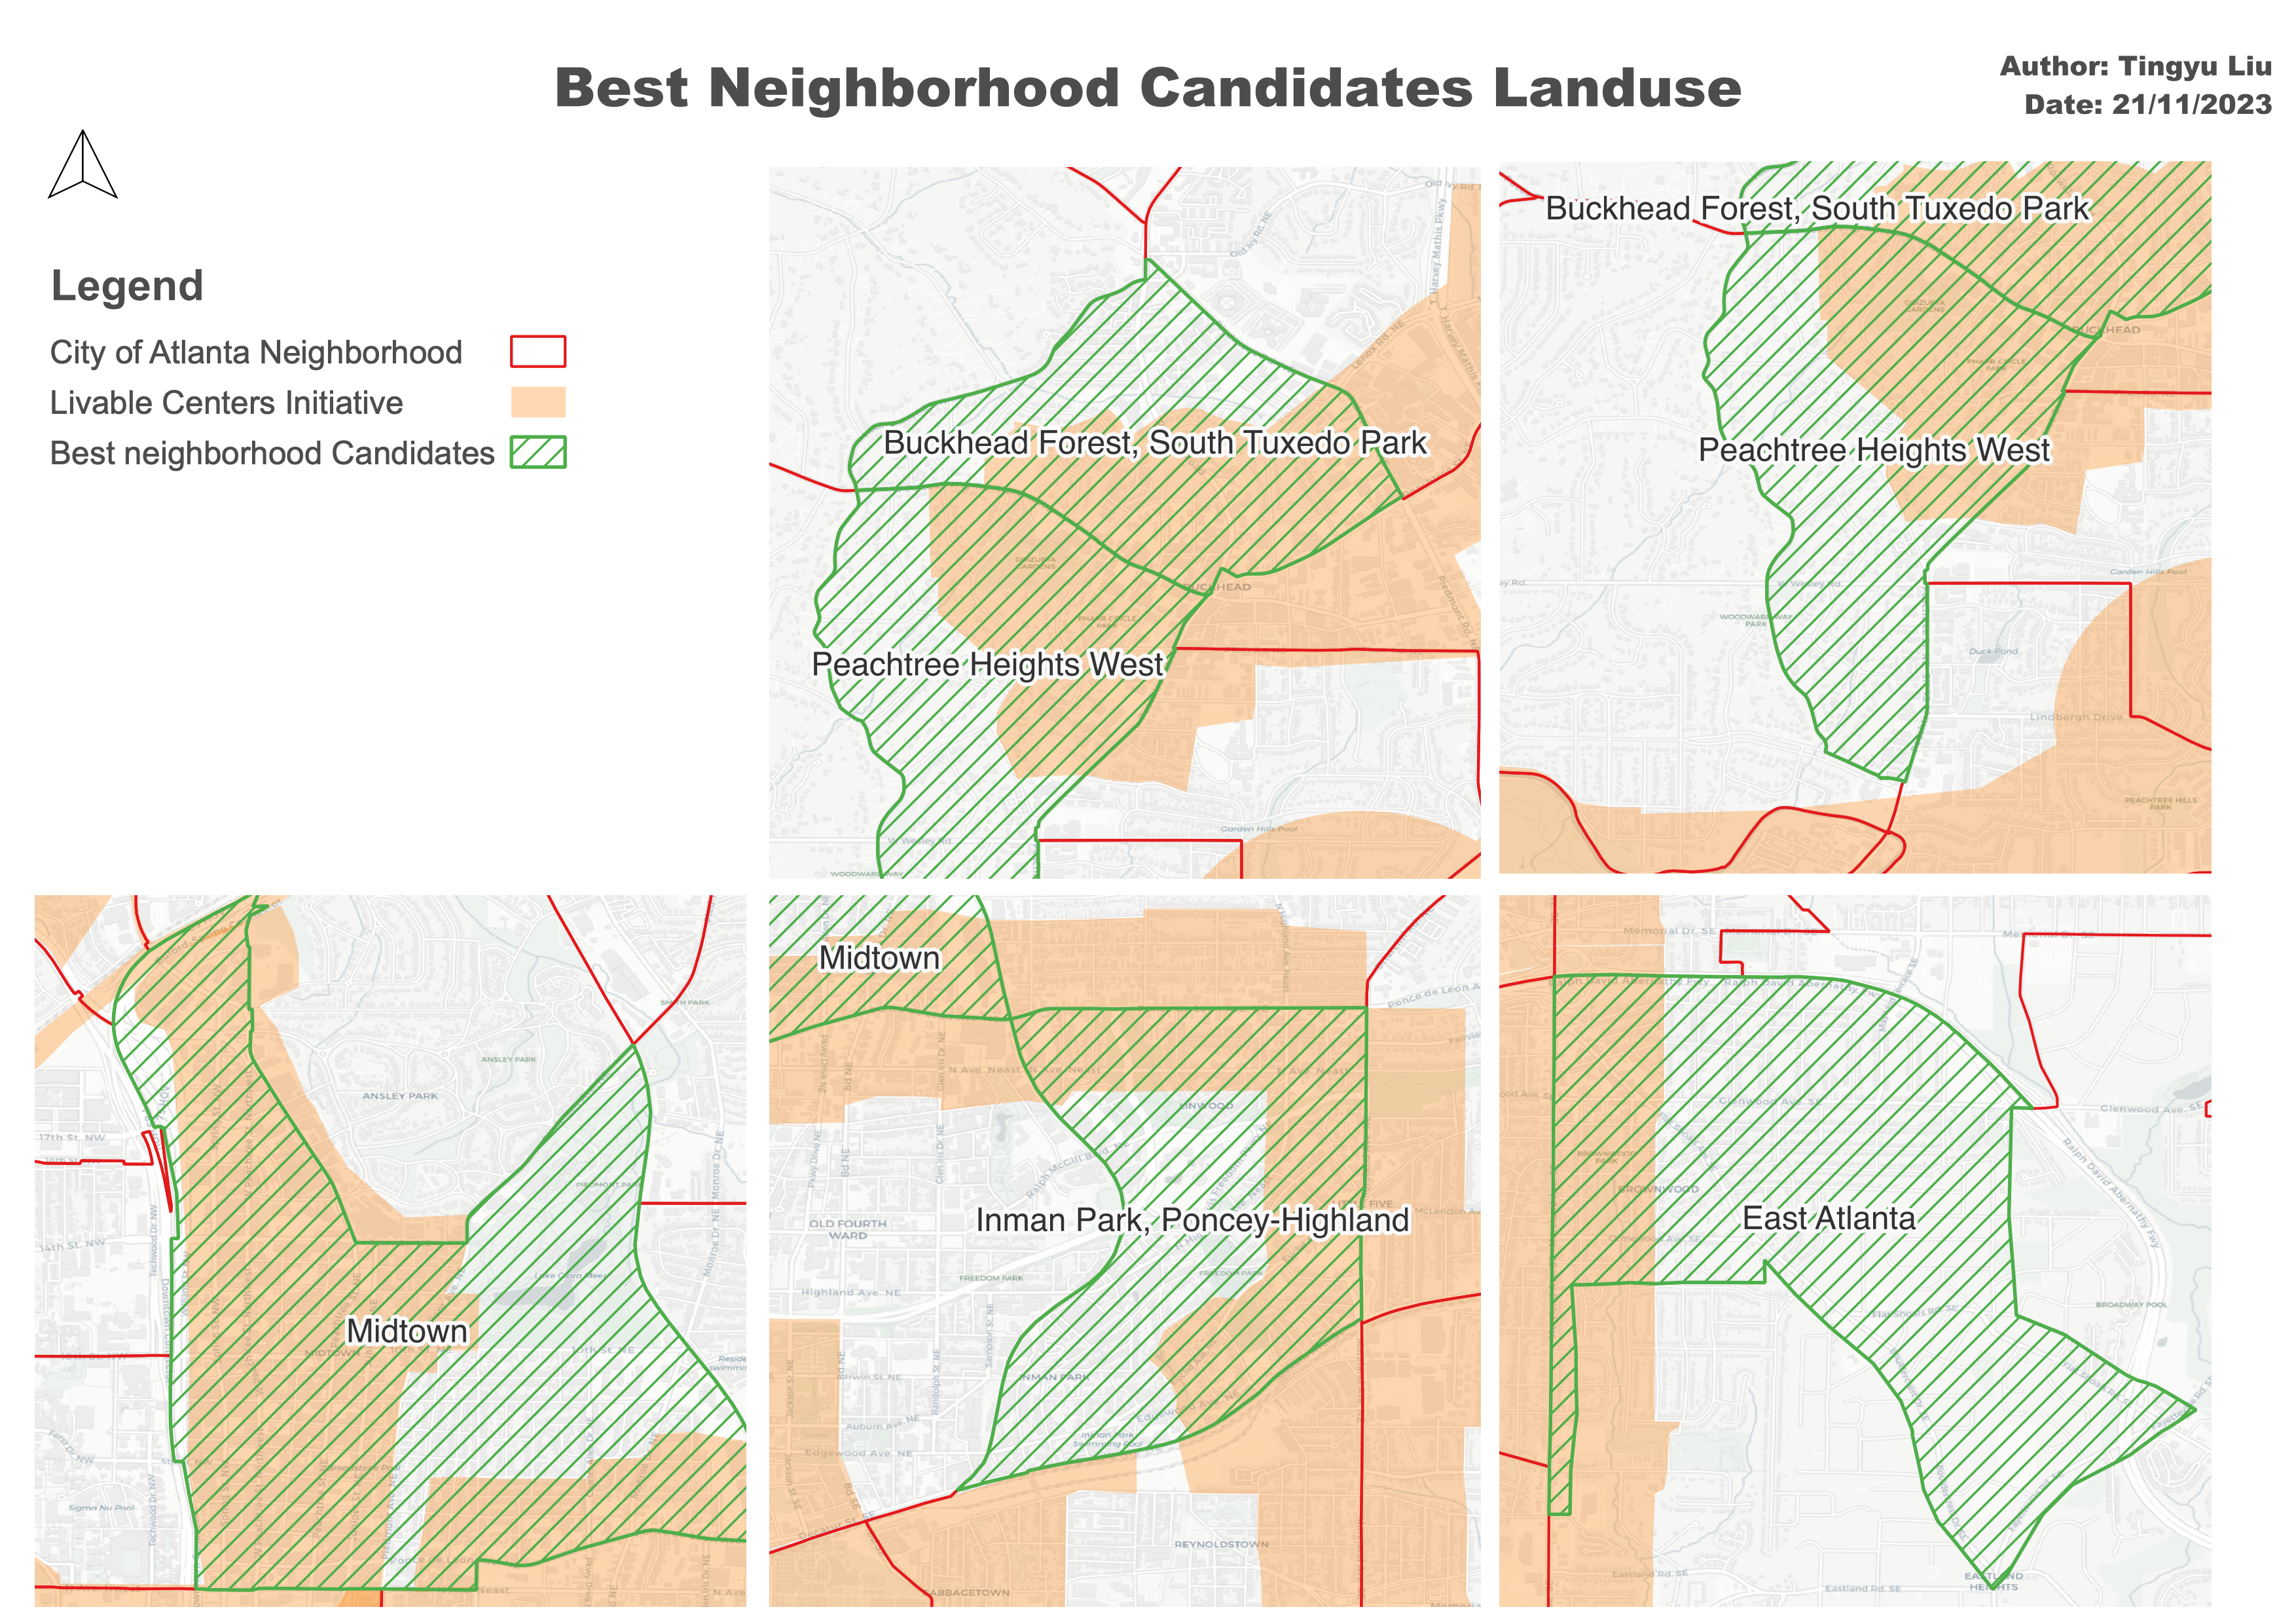
\includegraphics[width=0.7\textwidth]{map2/layout5- livable center restriction.png}
\caption{Figure 1: Different levels of urban development intensity}
\label{fig:figure1}
\end{center}
\end{figure}


\subsection{Conclusion}
After quantifying transport and demographic factors, and using transport and urban planning factors as restrictions, we have determined that Midtown and Inman Park are the best locations for a metal music venue business.

In more detail, Midtown has a more established music venue business and is more competitive. It will be more familiar to metalheads, but it is also a high-risk, high-reward type of venture.

Inman Park has higher potential with fewer existing music venues and suitable conditions for this business. Suggested location for music venue will be Edgewood Avenue, which has a restaurant street, however, the real estate price is also higher. 



\subsection{Discussion}




\textbf{Merits and Long-term Effects}
The merits and long-term effects of this project include promoting a vibrant music scene in Atlanta and providing valuable insights for businesses looking to establish a metal music venue in the city.

\textbf{Uncertainty and Error}
The uncertainty and error in this project could arise from the accuracy of the data sources and the assumptions made in the spatial and mathematical model.

\textbf{Data source Uncertainty and Error}







\newpage

\section{Reference}

{[}1{]} Florida, R., Jackson, S. (2010). Sonic City: The Evolving Economic Geography of the Music Industry. Journal of Planning Education and Research, 29(3), 310-321. https://doi.org/10.1177/0739456X09354453

{[}2{]} Castro, G. (2017, October 26). Mass Destruction Metal Fest Set to Put the Southeast on the Metal Map - Immersive Atlanta. Immersive Atlanta | Atlanta Music, Arts and Culture. https://immersiveatlanta.com/mass-destruction-metal-fest-set-to-put-the-southeast-on-the-metal-map/

{[}3{]} 2021 CDP - Atlanta Department of City Planning. (n.d.). Atlanta Department of City Planning. Retrieved December 10, 2023, from https://www.atlcitydesign.com/2021-cdp)

{[}4{]} Whiting, S. (2021). The Value of Small Live Music Venues: Alternative Forms of Capital and Niche Spaces of Cultural Production. Cultural Sociology, 15(4), 558-578. https://doi.org/10.1177/17499755211021307

{[}5{]} \textit{Carah, N., Regan, S., Goold, L., Rangiah, L., Miller, P., Ferris, J. (2021). Original live music venues in hyper-commercialised nightlife precincts: exploring how venue owners and managers navigate cultural, commercial and regulatory forces. International Journal of Cultural Policy, 27(5), 621-635. https://doi.org/10.1080/10286632.2020.1830979}

{[}6{]} Tai, Y. (2014). \textit{You Can't Always Get What You Want: Gatekeeping and Social Capital in the Live-Music Scenes of Atlanta and Taipei} (Order No. 3639931). Available from ProQuest Dissertations \& Theses A\&I; ProQuest Dissertations \& Theses Global. (1614473153). https://www.proquest.com/dissertations-theses/you-cant-always-get-what-want-gatekeeping-social/docview/1614473153/se-2

{[}7{]} Walser, R. (1993). Running with the devil: Power, gender, and madness in heavy metal music. Wesleyan University Press.

{[}8{]} Yelp Business Search API. (n.d.). Yelp. Retrieved from \textit{https://www.yelp.com/developers/documentation/v3/business\_search}

{[}9{]} Census Bureau API. (n.d.). U.S. Census Bureau. Retrieved from https://www.census.gov/data/developers/data-sets.html

{[}10{]} American Community Survey 5-year estimates for 2019. (n.d.). U.S. Census Bureau. Retrieved from https://www.census.gov/data/developers/data-sets/acs-5year.html

{[}11{]} Boeing, G. 2017. OSMnx: New Methods for Acquiring, Constructing, Analyzing, and Visualizing Complex Street Networks. Computers, Environment and Urban Systems 65, 126-139.

{[}12{]} Fulton County, Georgia. Open Data. Retrieved November 23, 2023, from https://gisdata.fultoncountyga.gov/

{[}13{]} Accuracy. (2020, December 28). OpenStreetMap Wiki, . Retrieved 20:12, December 10, 2023 from https://wiki.openstreetmap.org/w/index.php?title=Accuracy\&oldid=2079309.

{[}13{]} Shukla, A. (2022). The Social Psychology Of Heavy Metal \& Rock Music: Research On Metalheads. \textit{Cognition Today}. Retrieved September 19, 2022.











    % Add a bibliography block to the postdoc
    
    
    
\end{document}
